\documentclass[paper=a4, fontsize=11pt,twoside]{scrartcl} 

\usepackage[a4paper,pdftex]{geometry}
\setlength{\oddsidemargin}{5mm}
\setlength{\evensidemargin}{5mm}

\usepackage[english]{babel}
\usepackage[protrusion=true,expansion=true]{microtype}	
\usepackage{amsmath,amsfonts,amsthm,amssymb}
\usepackage{graphicx}

% --------------------------------------------------------------------
% Definitions (do not change)
% --------------------------------------------------------------------
\newcommand{\HRule}[1]{\rule{\linewidth}{#1}}

\makeatletter
\def\printtitle{
	{\centering \@title\par}}
\makeatother

\makeatletter
\def\printauthor{
	{\centering \large \@author}}
\makeatother

% --------------------------------------------------------------------
% Metadata
% --------------------------------------------------------------------
\title{
    \normalsize \textsc{Future Computing Technologies Lab: Creative Inquiry} \\ [2.0cm]
	\HRule{0.5pt} \\
	\LARGE \textbf{\uppercase{Semester Report}}
	\HRule{2pt} \\ [0.5cm]
	\normalsize \today
}

\author{
	Joel Miller\\	
	Clemson University\\	
	Department of Electrical and Computer Engineering\\
	\texttt{jmill53@clemson.edu} \\
}


% --------------------------------------------------------------------
% Main Document
% --------------------------------------------------------------------
\begin{document}

\thispagestyle{empty}

\printtitle
\vfill
\printauthor
\newpage

\setcounter{page}{1}

% Introduction
\section{Introduction}

This project focuses on predicting vehicle prices using a data set sourced from Kaggle. The analysis involves various steps, such as data cleaning, visualization, and model training. The data set is initially loaded using pandas, and a thorough exploration is conducted by examining its structure and content. Data cleaning steps include handling duplicate values and addressing missing or inconsistent entries.

% Data Cleaning and Exploration
\section{Data Cleaning and Exploration}

Duplicate values in the data set are identified and removed to ensure data integrity. Missing values are assessed, and necessary actions are taken to handle them appropriately. The data set's statistical characteristics, such as mean, median, and quartiles, are explored to gain insights into its numerical features.

% Feature Engineering
\section{Feature Engineering}

Several columns are dropped, and data types are adjusted to enhance model predictability. The age of vehicles is calculated based on the production year, and the data set is further refined by transforming columns like 'Mileage,' 'Engine volume,' and 'Levy' for better numerical representation.

% Data Visualization
\section{Data Visualization}

Various visualizations are employed to understand the distribution and characteristics of the data set. Histograms illustrate the distribution of numerical features, providing insights into variables such as mileage, engine volume, and age. Count plots display the frequency of categories within columns like 'Category,' 'Color,' and other categorical variables.

% Exploratory Data Analysis
\section{Exploratory Data Analysis}

In-depth exploratory data analysis is performed, revealing patterns and trends in the data set. The distribution of vehicles across different categories, colors, and features like leather interior, fuel type, gearbox type, drive wheels, and wheel are visualized to highlight key insights.

% Manufacturer Analysis
\section{Manufacturer Analysis}

The project delves into the most frequent vehicle manufacturers, providing a bar plot of the top 10 manufacturers. Additionally, the average prices of these top manufacturers are analyzed, offering further insights into the market.

% Price Analysis
\section{Price Analysis}

A scatter plot is utilized to assess the relationship between the 'Lien' (formerly 'Levy') and vehicle prices, providing insights into potential correlations.

% Correlation Analysis
\section{Correlation Analysis}

The correlation between numerical features is visualized using a heatmap, providing a comprehensive overview of the relationships within the dataset.

% Outlier Detection and Treatment
\section{Outlier Detection and Treatment}

Outliers in continuous features are identified through boxplots and treated to enhance the robustness of the data set.

% Data Transformation for Modeling
\section{Data Transformation for Modeling}

Object columns are converted to numerical format using label encoding, preparing the data set for model training.

% Linear Regression Model
\section{Linear Regression Model}

A Linear Regression model is implemented to predict vehicle prices. The model is trained on a subset of the data set, and its performance is evaluated using metrics such as R-squared and Root Mean Squared Error (RMSE).

% Conclusion
\section{Conclusion}

This project involves a comprehensive analysis of a vehicle pricing data set, encompassing data cleaning, visualization, and linear regression modeling. The insights gained from this analysis can inform decision-making processes in the automotive industry.


\begin{figure}[h!]
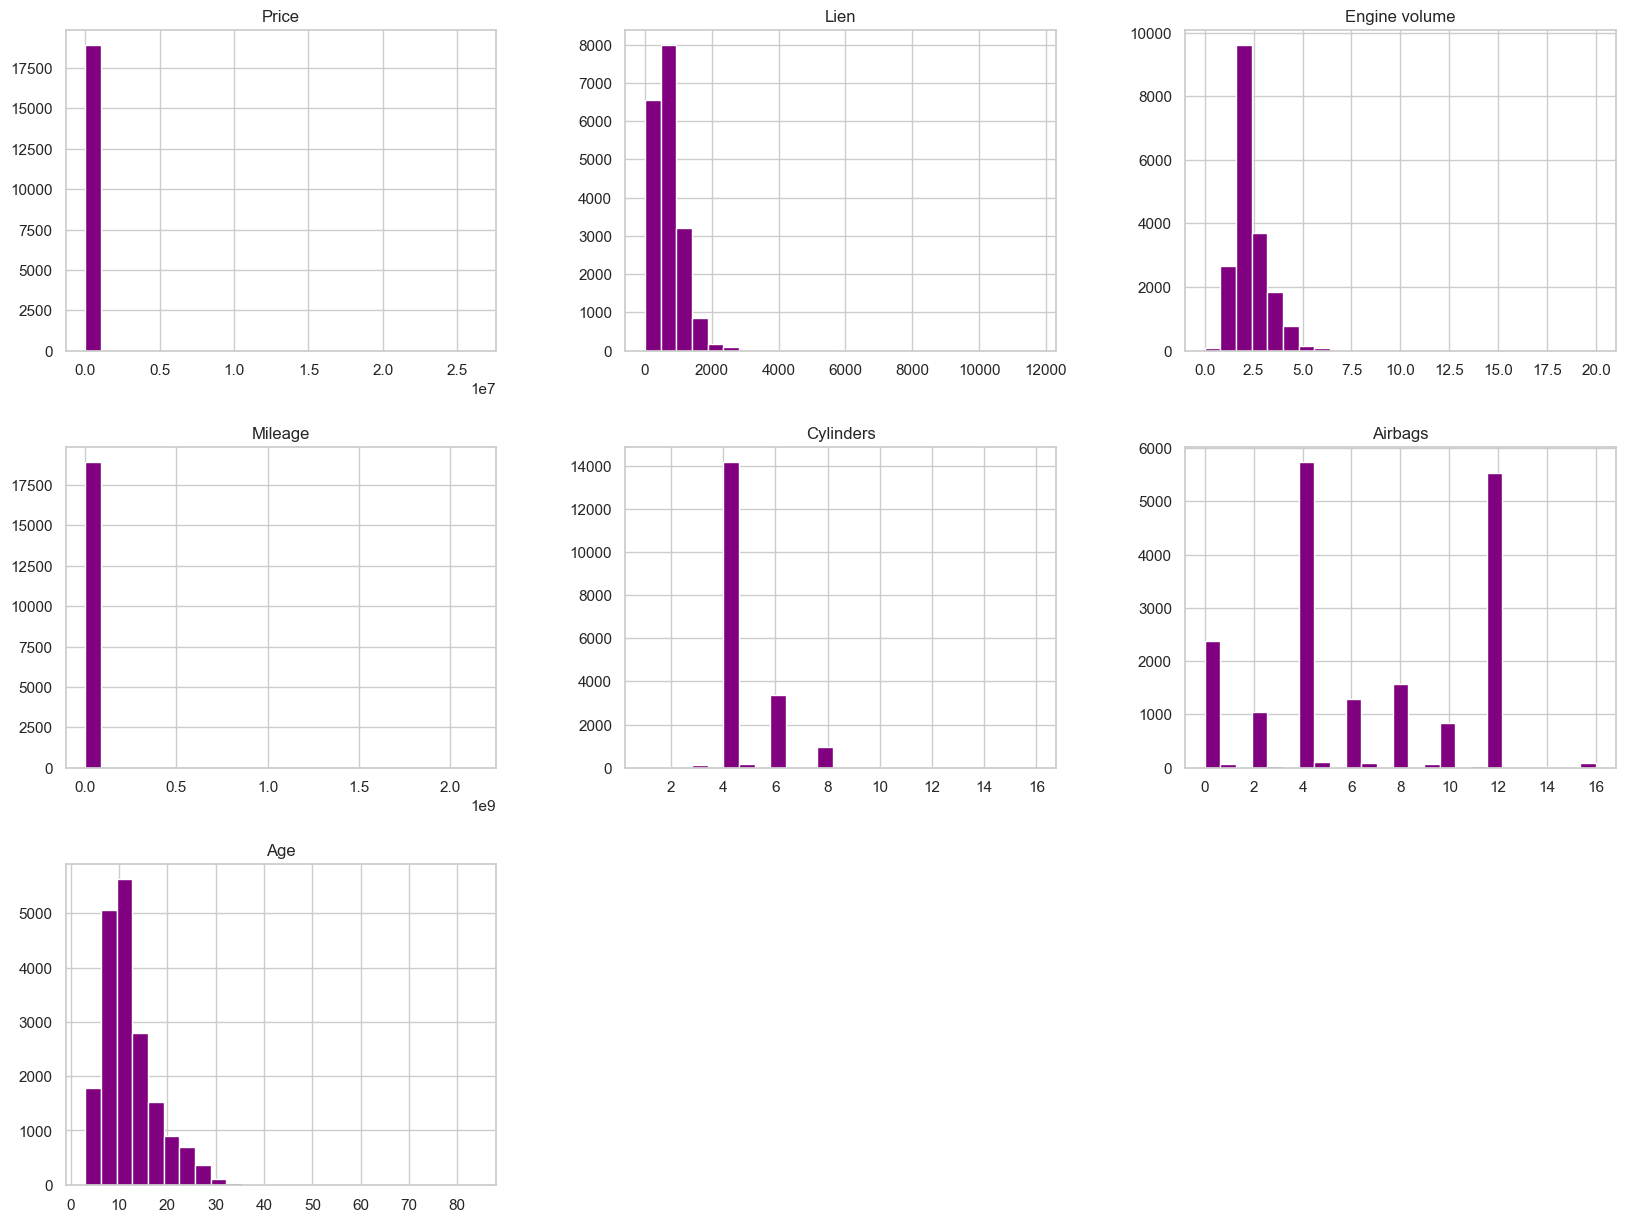
\includegraphics[width=\textwidth]{visual.png}
\caption{\label{fig:your-figure}Visual}
\end{figure}

\begin{figure}[h!]
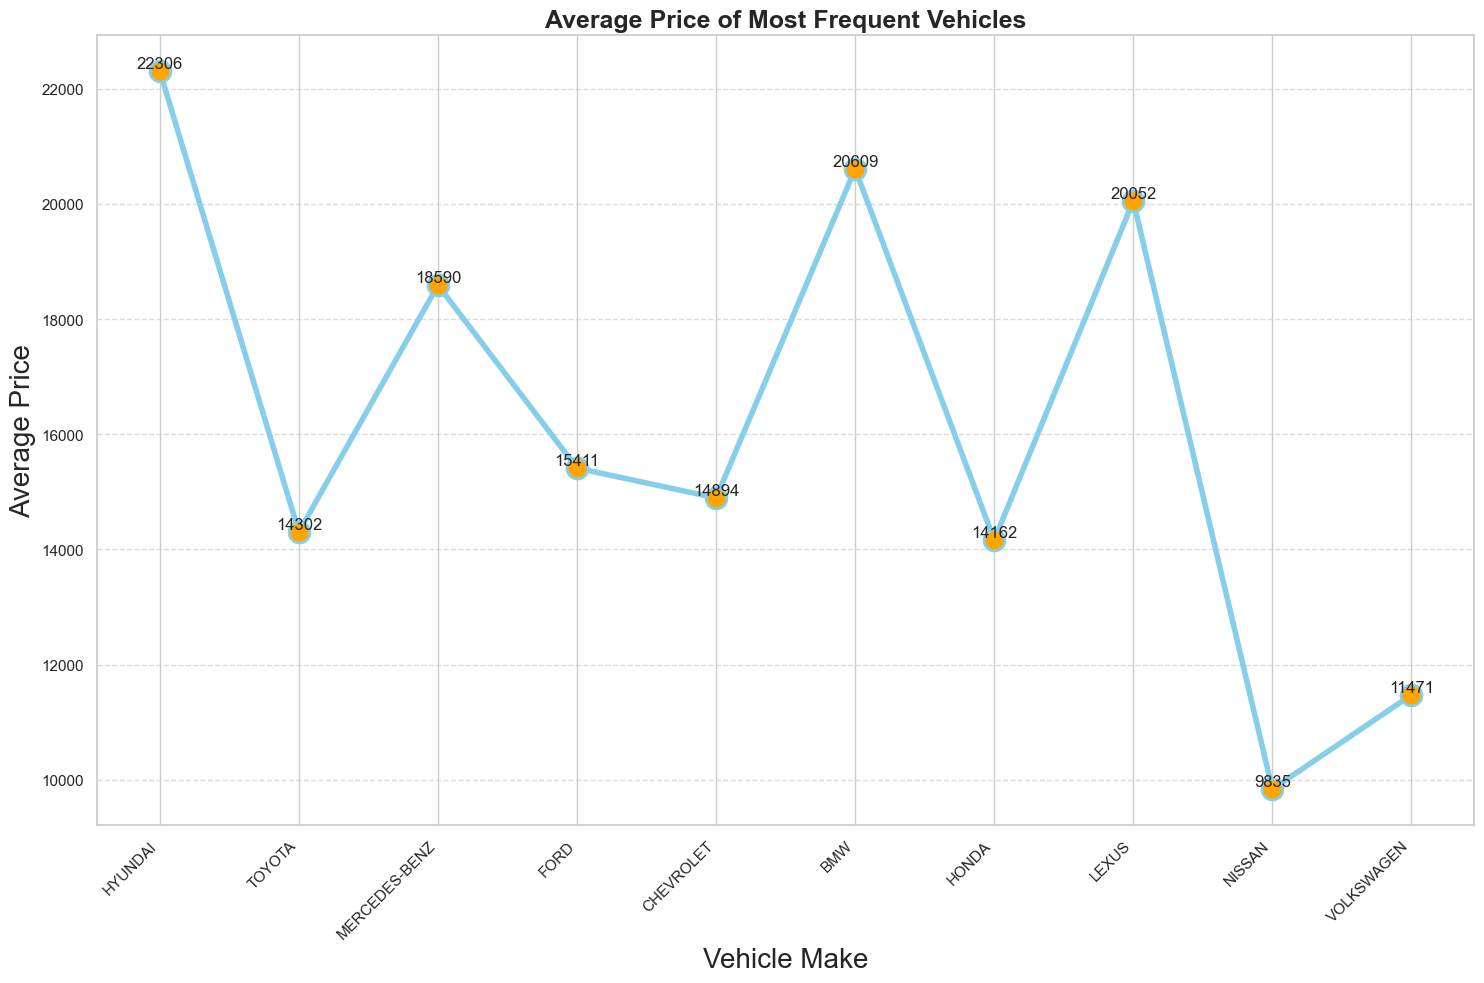
\includegraphics[width=\textwidth]{price.png}
\caption{\label{fig:your-figure}Prices}
\end{figure}


\begin{figure}[h!]
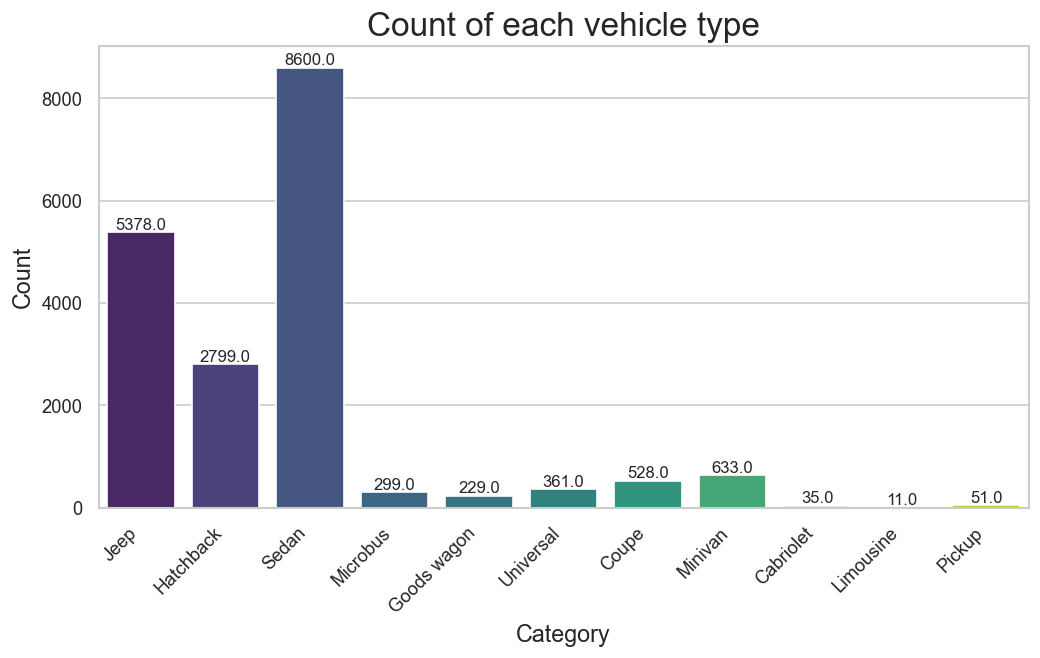
\includegraphics[width=\textwidth]{count.png}
\caption{\label{fig:your-figure}Counts}
\end{figure}


\begin{figure}[h!]
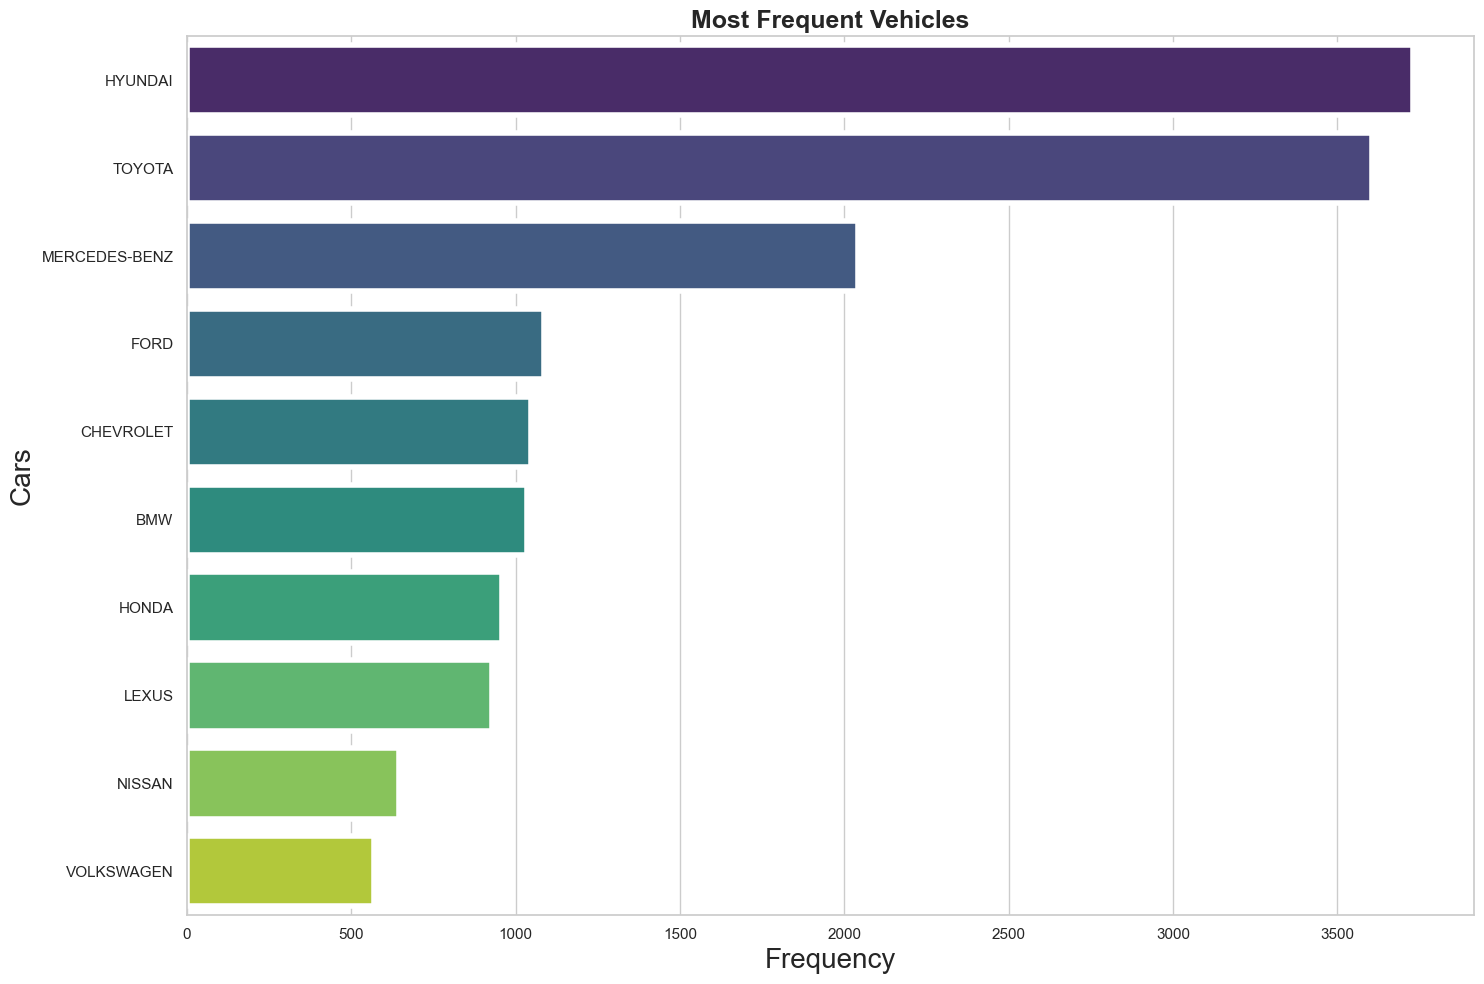
\includegraphics[width=\textwidth]{frequent.png}
\caption{\label{fig:your-figure}Frequency}
\end{figure}

\begin{figure}[h!]
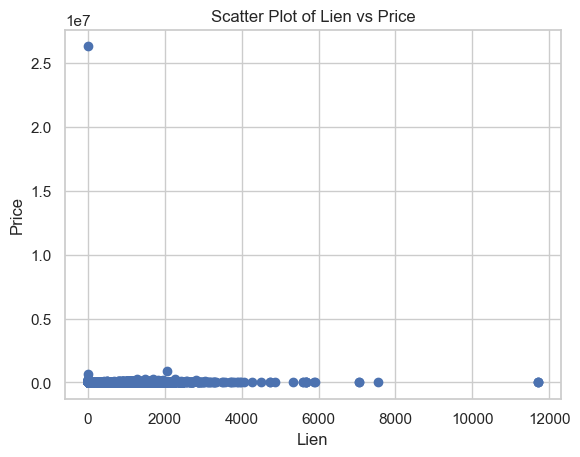
\includegraphics[width=\textwidth]{scat.png}
\caption{\label{fig:your-figure}Visual}
\end{figure}


\begin{figure}[h!]
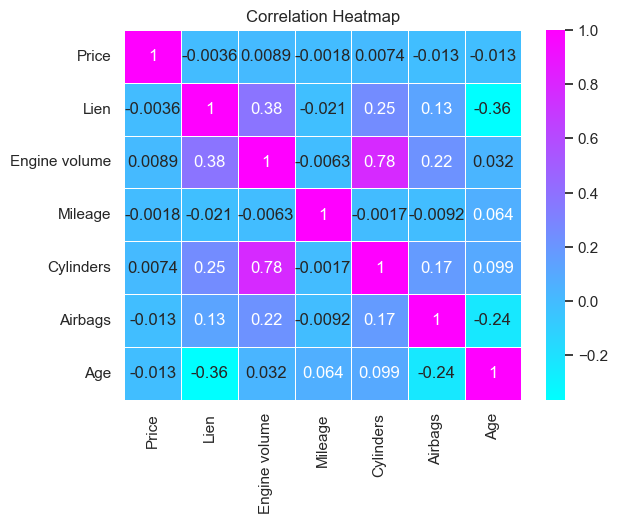
\includegraphics[width=\textwidth]{heat.png}
\caption{\label{fig:your-figure}Correlation Heat Map}
\end{figure}


\begin{figure}[h!]
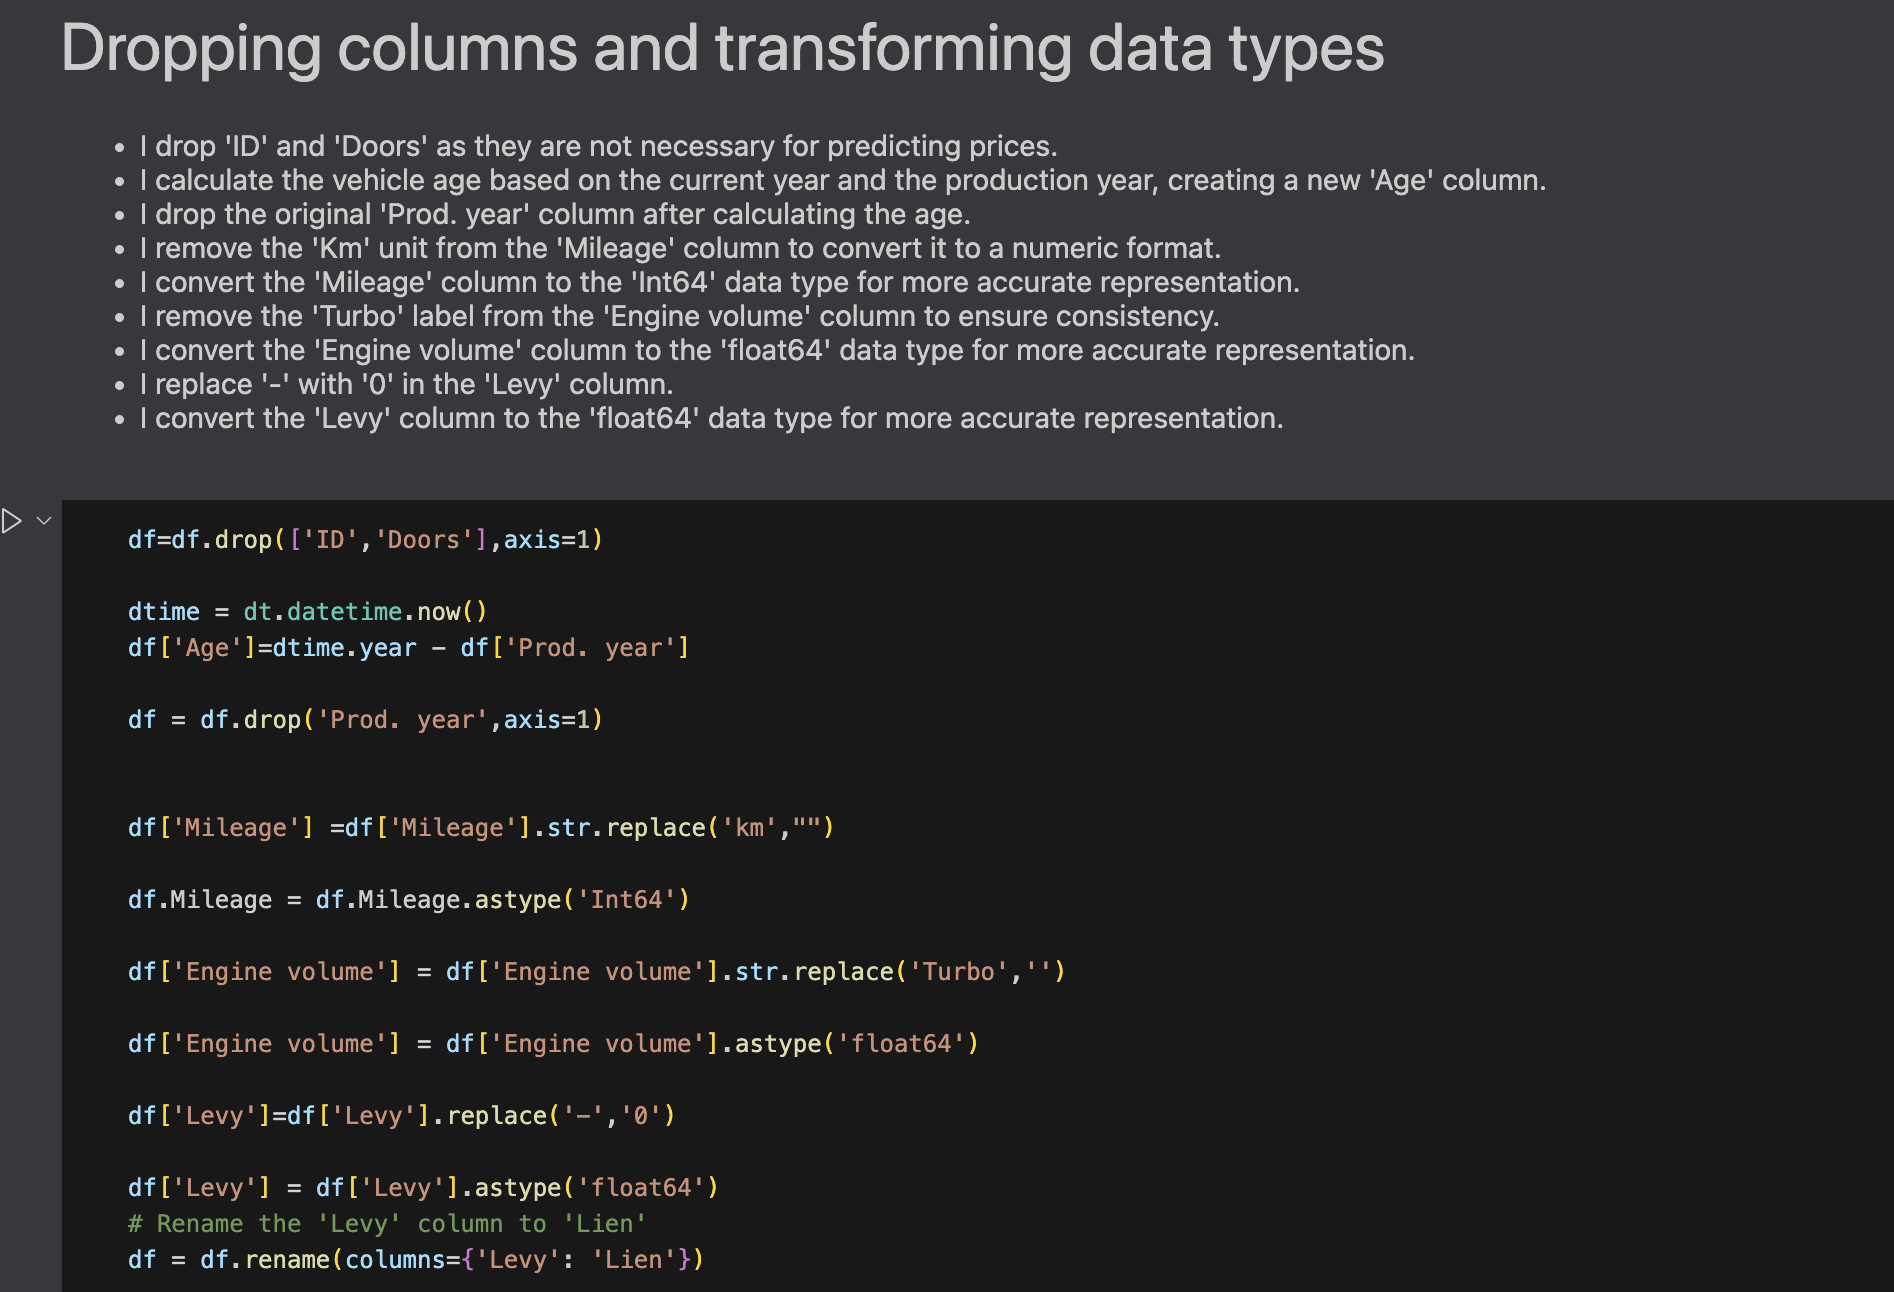
\includegraphics[width=\textwidth]{drop.png}
\caption{\label{fig:your-figure}Dropping Columns}
\end{figure}

\begin{figure}[h!]
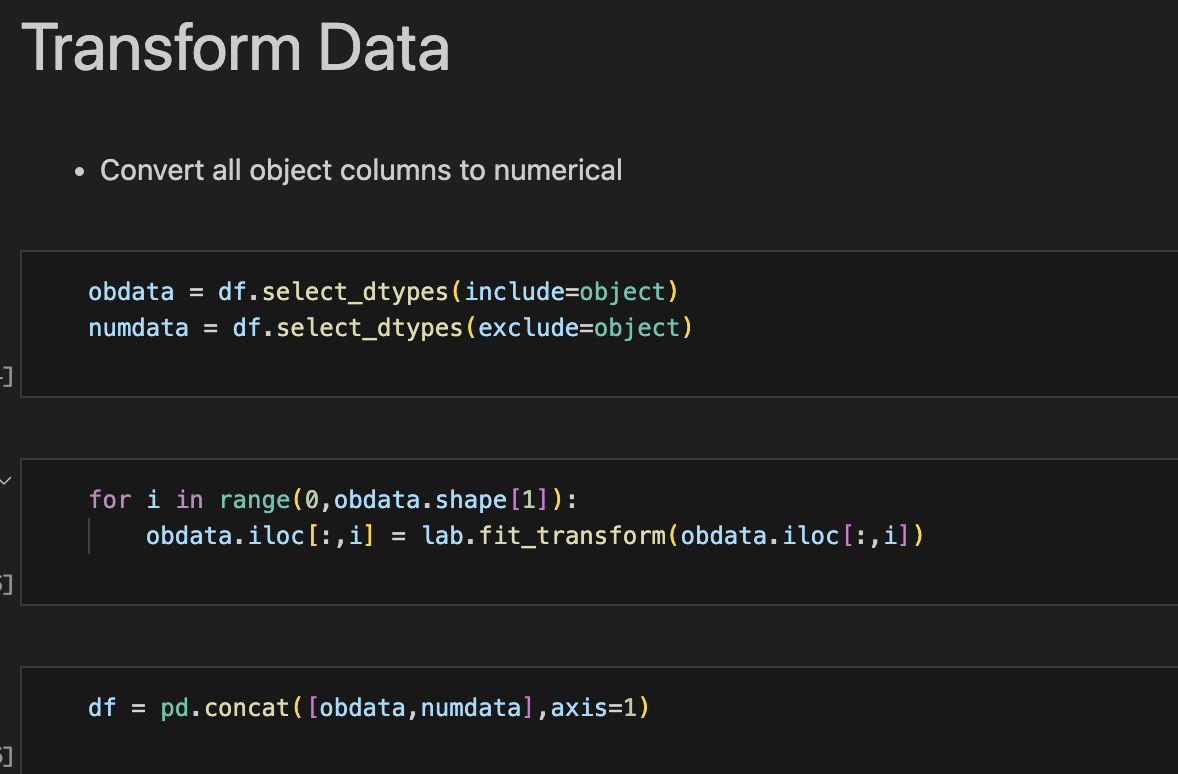
\includegraphics[width=\textwidth]{transform.png}
\caption{\label{fig:your-figure}Transforming Data}
\end{figure}

\begin{figure}[h!]
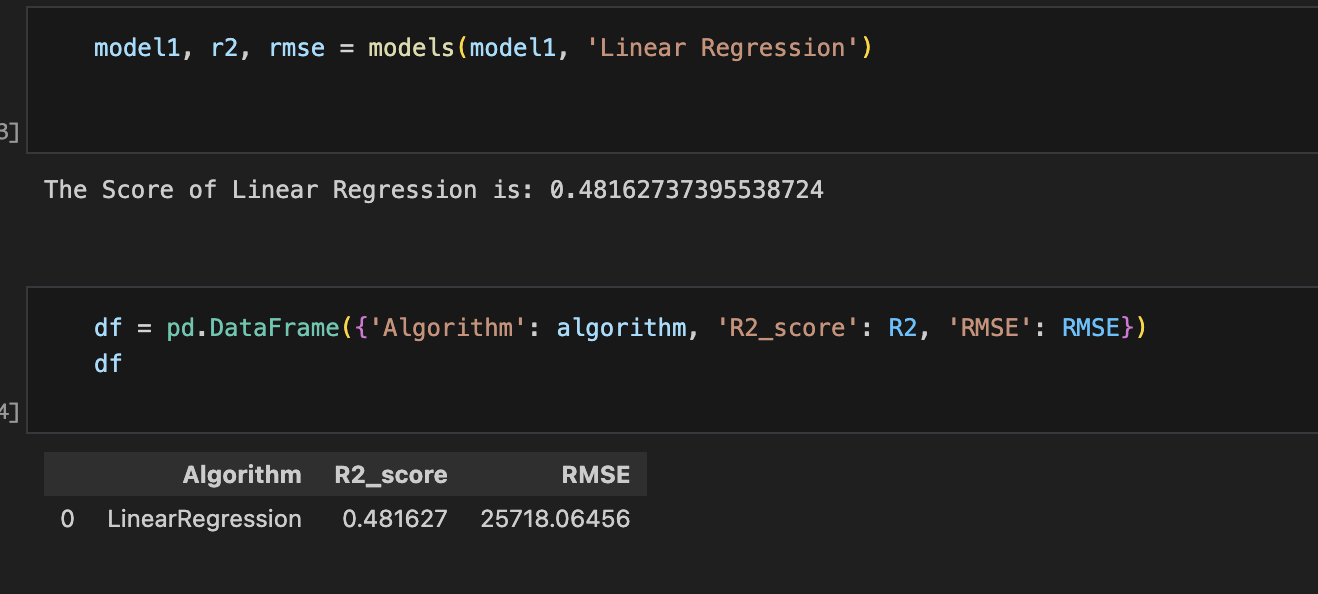
\includegraphics[width=\textwidth]{results.png}
\caption{\label{fig:your-figure}End Results}
\end{figure}





\end{document}
